\section{Background}
In this section, we present the necessary background knowledge about weights pruning and low-rank factorization. Note that we only focus on unstructured weights pruning since structured pruning is model architecture-dependent.
\subsection{Weights Pruning}
\label{sec:pruning}
We first establish some shared notations for different weights pruning algorithms. 
Let $\bm{W}\in \mathbb{R}^{n\times m}$ denote a generic weight matrix in a PLM. In order to determine which elements in $\bm{W}$ are pruned, an importance score matrix $\bm{S}\in \mathbb{R}^{n\times m}$ is correspondingly introduced. The smaller $S_{i,j}$ is, the larger the probability of $W_{i,j}$ will be pruned. Given the importance scores, a pruning strategy $f_{prune}(\cdot)$ computes a binary mask matrix $\bm{M}\in \{0,1\}^{n\times m}=f_{prune}(\bm{S})$, 
and the forward process for an input $x$ becomes $y=(\bm{W}\odot\bm{M})x$, 
where $\odot$ denotes element-wise multiplication.

\paragraph{Zero-order Weights Pruning} Zero-order weights pruning refers to the family of algorithms that only use the value of weight as a measure of importance.
For example, maginitude-based weights pruning~\cite{mag,chen2020lottery} adopts the absolute value of each weight as importance score, i.e., 
$\bm{S}_{i, j}=|\bm{W}_{i, j}|$. Then the typical choice of $f_{prune}(\cdot)$ is to remove $v\%$ percent of weights with smallest importance:
\begin{align}
	\bm{M}_{i,j}=
	\begin{cases} 
		0, & \text{if }\bm{S}_{i,j}~\text{is the smallest }v\%\\
		1,  & \text{otherwise}  
	\end{cases}
	\label{eq:zero}
\end{align}
Different sparsity can be obtained by varying $v$.

\paragraph{First-order Weights Pruning} Unlike zero-order weights pruning where $\bm{S}$ is directly derived from $\bm{W}$, first-order methods treate $\bm{S}$ as learnable parameters and jointly train it with model weights during fine-tuning. For example, soft-movement pruning~\cite{movement} implements $f_{prune}(\cdot)$ using a global threshold $\tau$:
\begin{align}
	\bm{M}_{i,j}=
	\begin{cases} 
		0, & \text{if }\bm{S}_{i,j}\le \tau\\
		1,  & \text{otherwise}  
	\end{cases}
	\label{eq:first}
\end{align}
Since the gradient of thresholding function is 0 everywhere, straight-through estimator~\cite{st} is used as approximation. The importance score $\bm{S}_{i,j}$ of $\bm{W}_{i,j}$ up to training step $T$ can be expressed as $\bm{S}_{i,j}=-\sum_{t\le T}(\frac{\partial \mathcal{L}}{\partial \bm{W}_{i,j}})^{(t)} \bm{W}_{i,j}^{(t)}$, where $\mathcal{L}$ is the loss function.
In this setting, different sparsity can be obtained by varying $\tau$.


\subsection{Low-rank Factorization}
\label{sec:lr}
Given the weight matrix $\bm{W}\in \mathbb{R}^{n\times m}$, low-rank factorization decomposes it into sub-matrices with fewer total amout of parameters to realize model compression.  It first uses singular value decomposition~(SVD) to obtain an equivalent form of $\bm{W}$ as the product of three matrices:
\begin{align}
	\bm{W}=\bm{U}\bm{\Sigma}\bm{V}^\mathrm{T}
\end{align}
where $\bm{U}\in \mathbb{R}^{n\times r}$, $\bm{\Sigma}\in  \mathbb{R}^{r\times r}$, $\bm{V}\in \mathbb{R}^{r\times m}$, and $r$ is the rank of matrix $\bm{W}$. $\bm{\Sigma}$ is a diagonal matrix of non-zero singular values $\{\sigma_1, \sigma_2,...,\sigma_r\}$ in descending order. Then, low-rank factorization with targeted rank $k$ is obtained by keeping the top-$k$ singular values in $\bm{\Sigma}$ as well as their corresponding column vectors in $\bm{U}$ and $\bm{V}$:
\begin{align}
	\bm{W}&\approx \bm{U}_{[:, :k]}\bm{\Sigma}_{[:k,:k]}\bm{V}_{[:, :k]}^{\mathrm{T}} \\
	&=\bm{A}\bm{B}
	\label{eq:svd}
\end{align}
where $\bm{A}=\bm{U}_{[:,:k]}\bm{\Sigma}_{[:k,:k]}$ and $\bm{B}=\bm{V}_{[:,:k]}^{\mathrm{T}}$ are the two final sub-matrices of which the product is used to replace $\bm{W}$. After such factorization, the number of parameters is reduced from $nm$ to $k(n+m)$. Different compression ratio can be achieved by varying preserved rank $k$.


\section{Preliminary Study}
\label{sec:pilot}
In this section, we conduct a preliminary study on low-rank factorization and weights pruning 
for compressing BERT into compact models, to provide some insights of these two methods.

\subsection{Experimental Setting}
\indent
\paragraph{Datasets}We use three NLU tasks SST-2, QNLI, and QQP as our evaluation testbeds. All of them are formulated as classification problem.

\paragraph{Examined Methods} For low-rank factorization, we follow the algorithm described in \secref{sec:lr}. Specifically, we first train pre-trained BERT to get the fine-tuned models for each task, following \citet{bert}. Then, we perform low-rank factorization on weight matrices of each linear layer in the fine-tuned BERT and re-trains the whole model to recover the lost accuracy. We empirically select $k$ from $\{120, 100, 80, 60, 40\}$.

For zero-order weights pruning, we choose post-training one-shot magnitude pruning~(POMP) and the Lottery Ticket Hypothesis~(LTH)~\cite{chen2020lottery}. POMP prunes away specified percent of weights in a fine-tuned model in one go while LTH adopts iterative magnitude pruning to progressively reach the target sparsity. For first-order methods, we opt for soft-movement pruning~(SMvP) and contrastive pruning~(CAP)~\cite{cap}. For all pruning algorithms, we tune the relevant hyper-parameters to obtain sparse BERT with at least $97\%$ performance of the densely fine-tuned BERT.

\subsection{Results and Analysis}

% Please add the following required packages to your document preamble:
% \usepackage{multirow}
% Please add the following required packages to your document preamble:
% \usepackage{multirow}
\begin{table}[h]
	\centering
	\scriptsize
	\begin{tabular}{l|l|lll}
		\toprule
		\multicolumn{2}{c|}{Model}                          & SST-2       & QNLI          & QQP           \\
		\midrule
		\multicolumn{2}{c|}{BERT-base}                           & 92.0~(100\%)        & 91.4~(100\%)          & 92.4~(100\%)          \\
		\midrule
		\multirow{2}{*}{0th}                      & POMP & 89.8(50\%) & 88.9(62\%) & 90.3(70\%) \\
		& LTH  & 89.5(30\%) & 89.7(40\%)   & 90.7(40\%)   \\
		\midrule
		\multirow{2}{*}{1st} & CAP  & 90.0(13\%) & 89.2(20\%)   & 90.4(7\%)   \\
		& SMvP & 89.7(10\%) & 89.2(19\%)   & 90.1(6\%)  \\
		\midrule
		\multicolumn{2}{l|}{SVD-120} & 88.9~(22\%)      &86.1~(22\%)      & 90.0~(22\%)       \\
		\multicolumn{2}{l|}{SVD-100}  & 85.7~(19\%)      & 85.4~(19\%)     & 88.9~(19\%)       \\
		\multicolumn{2}{l|}{SVD-80}  &85.3~(15\%)       & 83.8~(15\%)     &87.9~(15\%)        \\
		\multicolumn{2}{l|}{SVD-60}  & 85.2~(12\%)      &  80.8~(12\%)    & 86.7~(12\%)       \\
		\multicolumn{2}{l|}{SVD-40}  &  84.5~(8\%)     &  70.5~(8\%)    &  83.1~(8\%)      \\
		\bottomrule
	\end{tabular}
	\caption{Accuracy of weights pruning and low-rank 
factorization.
Numbers within parentheses are the percentage of parameters compared to the original BERT-base.}
	\label{table:pilot}
\end{table}
The results are summarized in \tabref{table:pilot}. Compared to zero-order POMP and LTH, CAP and SMvP are able to identify more sparse subnetworks inside PLM with similar performance. This is largely due to the use of more informative gradient-level signals during training. Despite having fewer effective parameters, weights pruning delivers better performance than low-rank factorization. This is mainly because the unstructured sparsity may allow for more flexible processing of input.

We also noted that, as the compression rate increases, the performance of low-rank factorization drops more rapidly. 
We hypothesize that the weight matrices of densely fine-tuned BERT are high-rank, 
hence leading to a large approximation error when $k$ is small. 
To verify this assumption, we compute the rank of all weight matrices in the 
fine-tuned BERT for SST-2, QNLI, and QQP. We found that the average rank of weight matrices 
on all three tasks is roughly 767, which is almost full-rank 
for BERT-base with a hidden vector size of 768. Therefore our hypothesis is confirmed.

The above observation motivate us to further explore how the ranks of sparse models 
are affected by different weights pruning algorithms. To this end, we compute the average rank 
of matrices in sparse models produced by all pruning algorithms described before. 
Results are shown in \tabref{table:rank}.
\begin{table}[th]
	\centering
	\scriptsize
	\begin{tabular}{l|l|lll}
		\toprule
		\multicolumn{2}{c|}{Model}                          & SST-2       & QNLI          & QQP           \\
		\midrule
		\multicolumn{2}{c|}{BERT-base}                           & 767.2        & 767.7          & 767.3          \\
		\midrule
		\multirow{2}{*}{0th}                      & POMP & 767.3 & 767.5 & 767.3 \\
		& LTH  & 767.4 & 767.6   & 767.2  \\
		\midrule
		\multirow{2}{*}{1st} & CAP  & 356.6 & 350.1  & 407.8  \\
		& SMvP & 296.4& 421.9  & 404.1  \\
		\bottomrule
	\end{tabular}
	\caption{Average rank of weight matrices after pruning.}
	\label{table:rank}
\end{table}

Both POMP and LTH produce sparse models that are 
as high-rank as densely fine-tuned BERT. In contrast, the family of first-order pruning algorithms, 
i.e., CAP and SMvP, are able to obtain sparse model with a much lower average rank~(see Appendix \ref{sec:appendixA} for more detail). 
There are two reasons for explaining such differences: (1) the way first-order pruning derives importance score reflects the extent to which model weights are departing from 0 throughout the training process, which is more accurate; (2) the $f_{prune}(\cdot)$ used by first-order pruning tends to prune away consecutive weights, hence being more likely to produce a low-rank matrix.
%This indicates that gradient information is essential for pruning algorithms to discover 
%the intrinsic low-dimensional representation of PLM on a specific task. 

%\KZ{Perhaps don't call it ``rank distribution''.
%Distribution seems to suggest the varying numbers are due to some statistical process. But they are actually
%the results of different algorithms.}

Given the competitive performance and low-rank structure of first-order pruning algorithms, 
we aim to explore the possibility of performing low-rank factorization on low-rank sparse models 
for model compression. As a sanity check of its feasibility, we quantitatively measure the 
quality of low-rank approximation with various preserved ranks $k$. 
\figref{fig:norm} shows that given a specific $k$, 
the sum of top-$k$ singular values of matrices produced by SMvP takes much larger portion of total values than fine-tuning, suggesting that we can reserve more information of low-rank sparse matrix given the same $k$. The reconstruction error~(measured by Frobenius norm of $\bm{W}-\bm{A}\bm{B}$) of SMvP is also significantly lower, implying a higher approximation quality. Therefore, we have reasons to expect that low-rank factorization on low-rank sparse models can effectively combine: (1) the good performance of first-order weights pruning; (2) direct memory and computation reduction by matrix decomposition.
\begin{figure}[t]
	\centering
	\scalebox{0.145}{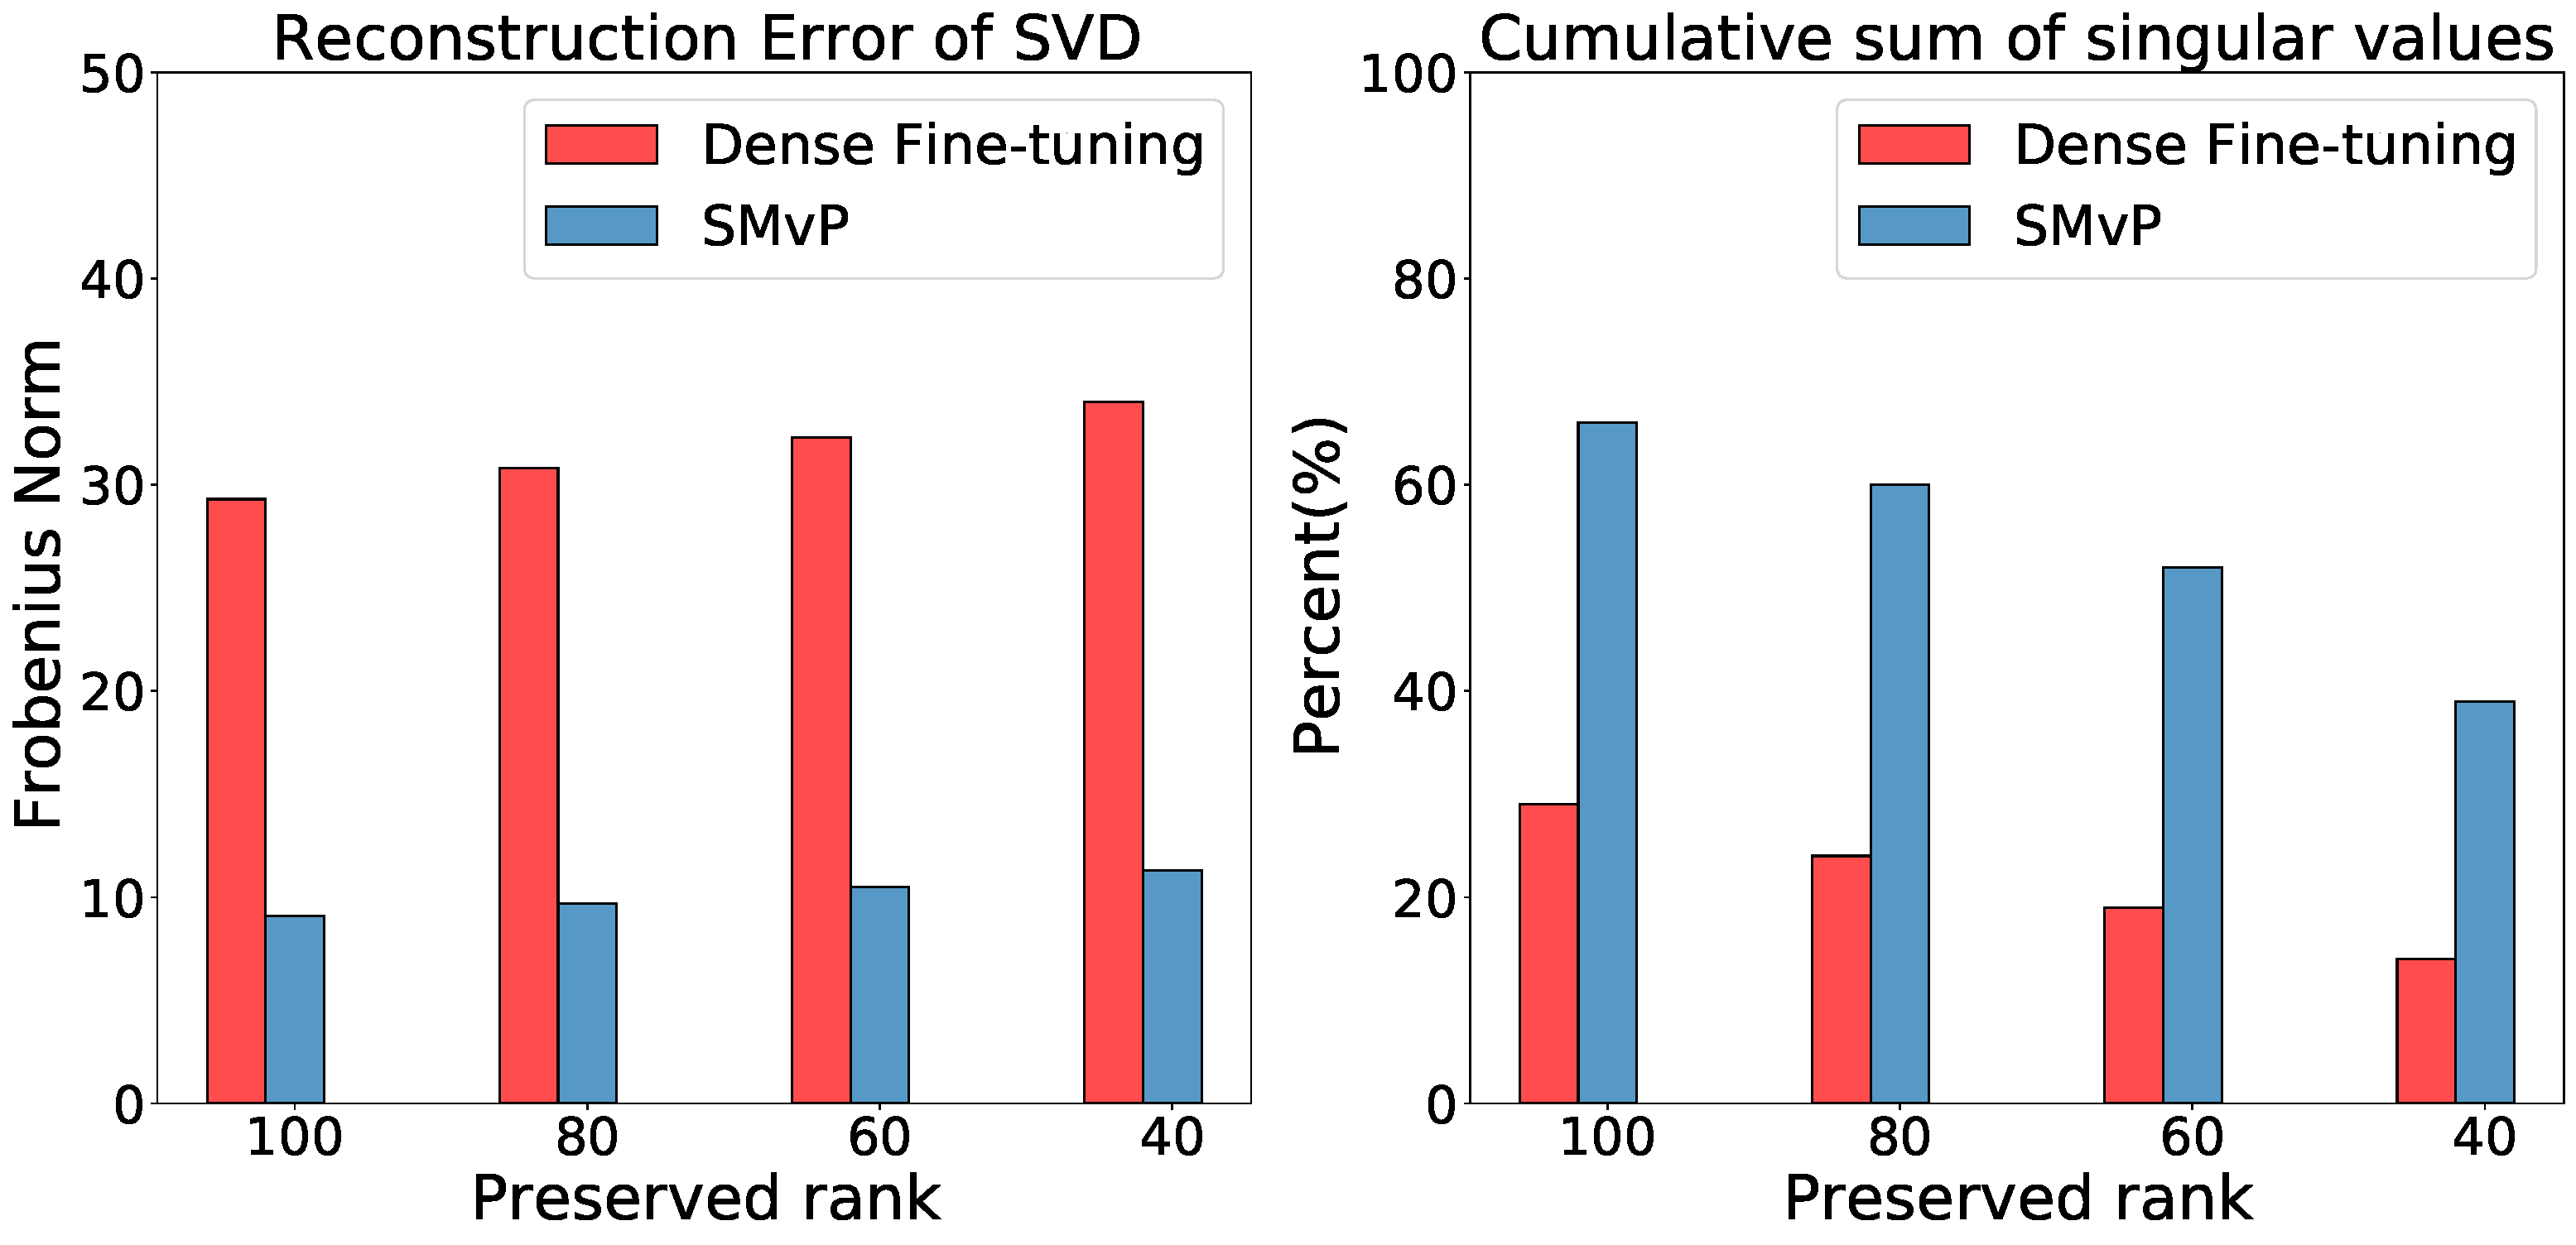
\includegraphics{./figures/norm_vis.pdf}}
	\caption{Quantitatively measuring approximation quality via reconstruction error~(left) and cumulative sum of singular values~(right) on QNLI.}
	\label{fig:norm}
\end{figure}


\section{Approach}
\label{sec:approach}
In this section, we formally introduce the proposed  
LPAF~(\textbf{L}ow-rank \textbf{P}rune-\textbf{A}nd-\textbf{F}actorize) framework 
%\KZ{I think the name of
%this method better carries ``low-rank'' in some way: Low-rank Prune-And-Factor (LPAF) (something
%that is pronouncable.} 
for language model compression. In addition, we propose two techniques that optimizes the 
initialization and training of the compression process.

\subsection{LPAF: Low-rank Prune-And-Factorize}
\label{sec:ptf}
Given a pre-trained language model $T$ and a downstream task with training set $D=\{(x_i, y_i), i=1,2,...N\}$, 
the first step of LPAF is to apply certain first-order pruning algorithm 
$P(\cdot, D, \alpha)$ to obtain the task-specific 
low-rank sparse model $T_{sparse}=P(T,D, \alpha)$. 
%\KZ{We gotta be careful with our wording: is it a framework or an algorithm? If it's a framework,
%then the first step 1st-order pruning algorithm can be substituted with any other such algo and
%the framework should still work well. Does our experiment support that? If we only show the results of
%SMvP then someone may say the good results are due to SMvP and not to our framework.}
Here $\alpha$ refers to the hyper-parameter that controls the trade-off between performance and sparsity, e.g., $\tau$ in SMvP and CAP. In this work, we instantiate $P$ with SMvP due to its training efficiency compared to CAP and report the results of LPAF using CAP in the Appendix \ref{sec:appendixC}.

Next, we apply SVD on each weight matrix~(excluding the embedding layer) in $T_{sparse}$ and 
obtain its low-rank factorized form $T_{factorized}=\text{SVD}(T_{sparse}, k)$ 
according to \eqnref{eq:svd}. The preserved rank $k$ is the only hyper-parameter determining the final compression rate. Finally, we re-train $T_{factorized}$ on $D$ with $\mathcal{L}_{task}$ until convergence, where $\mathcal{L}_{task}$ is the task-specific loss function.
\subsection{Sparsity-aware SVD}
\label{sec:sasvd}
SVD has been proven~\cite{bestsvd} to provide the optimal rank-$k$ approximation to $\bm{W}$ with respect to the Frobenius norm:
\begin{align}
	\nonumber
	\min_{\bm{A},\bm{B}} ||\bm{W}-\bm{A}\bm{B}||_{F}=\min_{\bm{A},\bm{B}} \sum_{i,j}(\bm{W}_{i,j}-(\bm{AB})_{i,j})^2
\end{align}
It is a generic factorization method in that it is applicable to any matrix $\bm{W}$ by penalizing the reconstruction error of each individual weight equally. 

In our case, $\bm{W}$ is a sparse matrix in which the majority of weights are set to zero by the pruning algorithm $P$. These zero weights are deemed to have less impact on the task performance compared to the retained~(unpruned) weights. 
To this end, we propose sparsity-aware SVD which considers different priorities of parameters and weighs the individual reconstruction error by multiplying with its importance score $S_{i,j}$:
\begin{align}
	\min_{\bm{A},\bm{B}}\sum_{i,j}\bm{S}_{i,j}(\bm{W}_{i,j}-(\bm{AB})_{i,j})^2
	\label{eq:sasvd}
\end{align}
In this way, parameters that are more important can be better reconstructed, hence retaining more task performance from $T_{sparse}$ at initialization. However, \eqnref{eq:sasvd} does not have a closed form solution~\cite{weightedsvd,hsu2021language} when each $\bm{W}_{i,j}$ has its own weight. We therefore resort to a simplification by letting the same row of $\bm{W}$ to share the same importance. The importance for row $i$ is given by $\hat{S}_{i}=\frac{\sum_{j}\bm{S}_{i,j}}{\sum_{n}\hat{S}_{n}}$. Let $\hat{\bm{I}}=diag(\hat{S}_1,\hat{S}_2,...,\hat{S}_{n})$ denote a diagonal matrix,  \eqnref{eq:sasvd} is now converted to:
\begin{align}
	\min_{\bm{A},\bm{B}}||\hat{\bm{I}}\bm{W}-\hat{\bm{I}}\bm{A}\bm{B}||_F
\end{align}
This essentially amounts to applying rank-$k$ SVD upon $\hat{\bm{I}}\bm{W}$, i.e., $\hat{\bm{I}}\bm{W}=\hat{\bm{U}}\hat{\bm{\Sigma}}\hat{\bm{V}}^\mathrm{T}$. Then the solution of $\bm{A}$ and $\bm{B}$ can be analytically obtained by:
\begin{align}
	\bm{A} &= \hat{\bm{I}}^{-1}\hat{\bm{U}}_{[:,:k]}\hat{\bm{\Sigma}}_{[:k,:k]},\bm{B}=\hat{\bm{V}}_{[:,:k]}^{\mathrm{T}}
\end{align}


\subsection{Mixed-rank Fine-tuning}
As introduced in \secref{sec:ptf}, the last step of LPAF is to fine-tune $T_{factorized}$ on the training set $D$. This process has been proven essential to regain the performance lost during factorization~\cite{svd}. However, during the experiments, we observe the performance of fine-tuned $T_{factorized}$ still slightly lags behind $T_{sparse}$ given similar parameter budget. 
%\KZ{Isn't it normal for $T_{factorize}$ to lag behind $T_{sparse}$? Is there any evidence (experimental results) to show
%this ``lagging''?  Even in Fig. 3, in most cases, $T_{sparse}$ is still better Ours. 
%So I don't see enough motivation for this Mixed-rank fine-tuning.} 
We posit that, due to the reduced model capacity, joint fine-tuning of low-rank weight matrices may converge to sub-optimal solutions with lower generalization ability. To mitigate this problem, we propose mixed-rank fine-tuning, a regularized scheme for training low-rank matrices.

Let $\{(\bm{A}\bm{B})_i, i=1,2...,N\}$ denotes all low-rank matrices in $T_{factorized}$. During training, for each $(\bm{A}\bm{B})_i$, we sample a binary Bernoulli random variable $z_i\sim \text{Bernoulli}(p)$, where $p$ is a global hyper-parameter. Then, the local computation process involving $(\bm{A}\bm{B})_i$ is modified to:
\begin{align}
	\bm{x}_{out} = (1-z_i)*(\bm{A}\bm{B})_i \bm{x}_{in} + z_i * \bm{W}_i\bm{x}_{in}
\end{align}
where $\bm{W}_i$ is the sparse matrix in $T_{sparse}$ from which $\bm{A}_i$ and $\bm{B}_i$ are derived. In this way, the low-rank matrices can additionally benefit from gradient-level supervision from  $T_{sparse}$, hence reducing the generalization gap. Due to the randomness introduced by sampling, the performance may have a large variance. To further stabilize training, we make each input data go through the forward pass twice with different $\bm{z}^1=\{z_i^1\}_{i=1}^{N}$ and $\bm{z}^2=\{z_i^2\}_{i=1}^{N}$, and impose a consistency objective on the two outputs:
\begin{align}
	\mathcal{L}_{c}=\mathcal{D}(y_{\bm{z}^1}, y_{\bm{z}^2})
\end{align}
where $\mathcal{D}$ measures the divergence between outputs from two forward passes. $\mathcal{D}$ can be the Kullback-Leibler divergence for classification tasks and  the mean-square-error for regression tasks.

The hyper-parameter $p$ is controlled by a scheduler. We implement it such that $p$ is linearly decayed from an initial value $p_{init}$ to zero by a constant step size $d$:
\begin{align}
	p = \text{max}(0, p_{init}-d*t)
\end{align}
After $p$ reaches zero, the training process then degenerates to R-Drop~\cite{rdrop} and the model still benefits from the regularization effect brought by different dropout masks.
